\documentclass[addpoints,12pt]{exam}
\usepackage{amsmath}
\usepackage{amsthm}
\usepackage{amsfonts}
\usepackage{systeme}
\usepackage{graphicx}
\usepackage{caption}
\usepackage{xfrac}
\usepackage{physics}
\usepackage{microtype}
\usepackage{eulervm}
%\usepackage[framemethod=tikz]{mdframed}
\usepackage{thmtools}
\usepackage{etoolbox}
%\usepackage{fouriernc}
\usepackage{mdframed}
\usepackage[overload]{empheq}
\usepackage{adjustbox}
\usepackage{enumitem}
\usepackage[explicit]{titlesec}
% adds in \varnothing for empty set
\usepackage{amssymb}
% adds in formated SI units
%\usepackage{siunitx}
\usepackage{pgfplots}
\usepackage{multirow}
\usepackage{array}

\pagestyle{headandfoot}
\runningfootrule
\firstpageheadrule
\runningheadrule

\newcommand{\class}{Math 0098}
\newcommand{\sem}{2211}
\newcommand{\due}{}
\newcommand{\sect}{11.1}
\newcommand{\topic}{The Quadratic Formula}

\firstpageheader{\class}{\sect - \topic}{}
\runningheader{\class}{\sect - \topic}{}
\firstpagefooter{\class}{}{Page \thepage\ of \numpages}
\runningfooter{\class}{}{Page \thepage\ of \numpages}

\newif\ifprintselected
\printselectedtrue
%\printselectedfalse

\newenvironment{select}
{\ifprintselected
	\printanswers
	\fi
}
{}

\theoremstyle{definition}
\newtheorem{theorem}{Theorem}
%\newtheorem{example}{Example}[subsection]
%\newtheorem{definition}{Definition}
%\newmdtheoremenv{definition}{Definition}[subsection]
%\newmdtheoremenv{example}{Example}[subsection]
\AtBeginEnvironment{defn}{\begin{minipage}{\textwidth}}
\AtEndEnvironment{defn}{\end{minipage}}
%\AtBeginEnvironment{example}{\begin{minipage}{\textwidth}}
%\AtEndEnvironment{example}{\end{minipage}}
\newcommand{\iu}{{i\mkern1mu}}

\setlength{\gridsize}{5mm}
\setlength{\gridlinewidth}{0.1pt}

\printanswers
\DeclareMathSizes{12}{12}{12}{12}

%%%%%%%%%%%%%%%%%%%%%%%%
% Create bars around subsubsection
%%%%%%%%%%%%%%%%%%%%%%%%

\titleformat{\subsubsection}
   {\large\bfseries}% format
   {}% label
   {0pt}% sep
   {\titlerule \vspace{.1in} #1}% before code
      [{\titlerule[0.4pt]\vspace{.1in}}]% after code
\titlespacing{\subsubsection}
   {0pt}% left
   {0pt}% before sep
   {\baselineskip}% after sep
   
%%%%%%%%%%%%%%%%%%%%%%%
% Create line break after definition label
%%%%%%%%%%%%%%%%%%%%%%%   
\newtheoremstyle{break}
  {\topsep}{\topsep}%
  {}{}%\itshape
  {\bfseries}{}%
  {\newline}{}%
\theoremstyle{break}
\newmdtheoremenv{definition}{Definition}[subsection]
\theoremstyle{break}
\newtheorem{example}{Example}[subsection]

%%%%%%%%%%%%%%%%%%%%%%
% start document
% set section, subsection (use n-1 for sub)
%%%%%%%%%%%%%%%%%%%%%%


\begin{document}
\setcounter{section}{11}
\setcounter{subsection}{1}

\subsection{The Quadratic Formula}
In the last section, we added the method \emph{completing the square} to our arsenal of tools to solve quadratic equations. Every tool that we have seen so far has had the downside of only working for a specific case of quadratics. This section introduces the method that trumps all others -- \emph{the quadratic formula}. While unwieldy and occasionally time consuming, the quadratic formula works in \emph{all} cases and will directly give you the solutions of a quadratic equation. We will also discuss a specific part of the quadratic formula, namely the \emph{discriminant} and discuss how it is used to categorize the solutions of an equation before we calculate them.
\vspace{.2in}
\begin{mdframed}
\textbf{The Quadratic Formula}
Given a quadratic equation written in the form $ax^2+bx+c=0$ with $a\neq 0$, the solutions of the equation are given as \[x = \dfrac{-b\pm\sqrt{b^2-4ac}}{2a}\]
\end{mdframed}

\vspace{.2in}

\begin{example}
Use the quadratic formula to solve the following:\[2x^2+9x-5=0\]

\end{example}

\newpage


\begin{example}
Use the quadratic formula to solve the following:\[2x^2=6x-1\]
\vspace{3.5in}
\end{example}
\begin{example}
Use the quadratic formula to solve the following:\[3x^2+5=-6x\]
\vspace{3.5in}
\end{example}

\newpage

\subsubsection*{The Discriminant}

The discriminant is the radicand in the quadratic formula. Typically we use the Greek letter $\Delta$ (delta) to represent the discriminant and define it as $\Delta = b^2-4ac$. We are able to use the determinant to determine what type of solutions an equation will have without actually solving for the solutions. In a class such as this, the discriminant isn't the most useful of tools, but it turns out that in higher level math classes the discriminant is invaluable.

\vspace{.2in}

\begin{figure}[h]
\centering
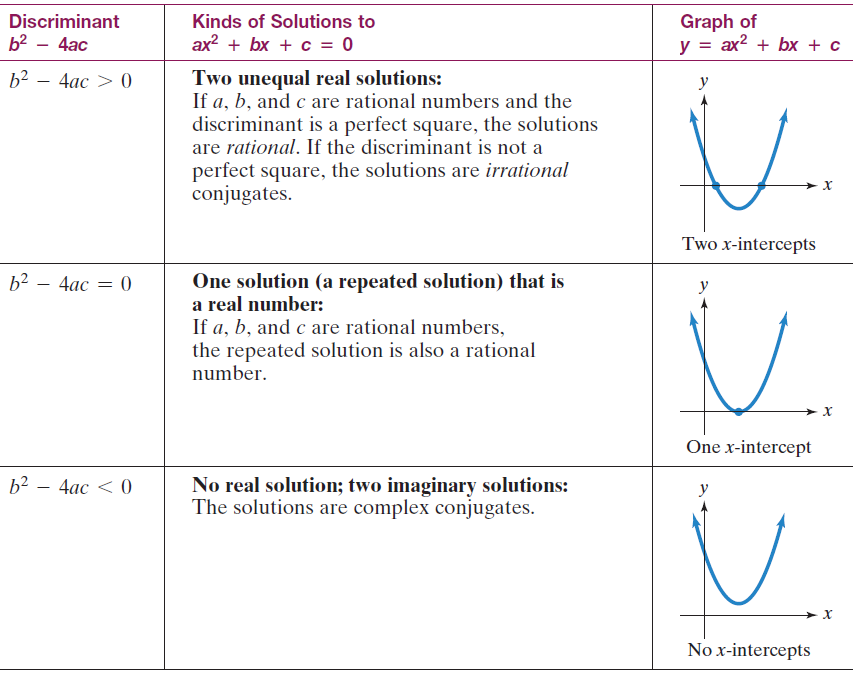
\includegraphics[scale=.7]{images/11_2_discriminant_table}
\end{figure}

\newpage

Using the discriminant is a fairly straightforward process. Start by calculating the discriminant ($\Delta = b^2-4ac$) and then identify the category from the given table into which it falls.

\vspace{.2in}

\begin{example}
Use the discriminant to classify the types of solutions each equation has:
\begin{enumerate}
\item $x^2+6x+9=0$
\vspace{1.75in}
\item $2x^2-7x-4=0$
\vspace{1.75in}
\item $3x^2-2x+4=0$
\vspace{1.75in}
\end{enumerate}
\end{example}

\newpage

\subsubsection*{Working Backwards -- Equations from Solutions}

We know that in the process of factoring and solving a quadratic equation, we typically end up with a line that looks like $(x-a)(x-b)=0$ which we then break apart and solve yielding solutions of $x=a$ and $x=b$. However, what if we know the solutions and want to determine an equation that has those solutions? Notice than I say \emph{an} equation. It is possible for there to be an infinite number of equations all with the same solutions.

\vspace{.2in}

\begin{mdframed}
\textbf{Working Backwards}
If we have solutions given by $x=a$ and $x=b$, start by setting $(x-a)(x-b)=0$ regardless of what $a$ and $b$ are (they could be whole number, decimals, radicals, fractions, imaginary, complex, etc.). Then, FOIL the expression and rewrite in standard form. You can obtain other equations that have the same solutions by multiple (or dividing) the equation by some value.
\end{mdframed}

\vspace{.2in}

\begin{example}
Find a quadratic equation with each of the following as roots:
\begin{enumerate}
\item $x = -\sfrac{3}{5}, x=\sfrac{1}{4}$
\vspace{2in}
\item $x = -5\sqrt{2}, x=5\sqrt{2}$
\end{enumerate}
\end{example}

\newpage

\begin{example}
Find a quadratic equation with the root $-7\iu$.
\vspace{2in}
\end{example}

\begin{example}
Find a \emph{cubic} equation with the roots $0, 1$ and $3$.
\vspace{2in}
\end{example}

\begin{example}
Find a \emph{cubic} equation with the roots $-1,1$ and $2$.
\end{example}
\end{document}